
\hypertarget{menu_edit}{}
\section{Edit}
\index{edit menu}
\index{RTF formatted}
\index{Export!RTF formatted}

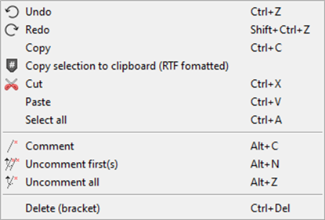
\includegraphics[scale=0.8]{./res/menu_edit.png}\\

\begin{scriptsize}
  \begin{tabularx}{\textwidth}{>{\hsize=0.4\hsize}X>{\hsize=0.7\hsize}X}\\
    \hline
    \textbf{Option} & \textbf{Description} \\
    \hline
    Undo & Undoes the last action \\
    Redo & Re-applies any actions undone using the Undo option \\
    Copy & Copies the selected text and places it in the Windows clipboard \\
    Copy selection to clipboard (RTF formatted) & Exports a selection to the Windows clipboard in RTF format.
     Useful for documenting R code in RTF editors. \\
    Cut & Cuts the selected text and places it in the Windows clipboard \\
    Paste & Places any text in the Windows clipboard at position indicated by the cursor within the file \\
    Select all & Selects the whole text contained in the file \\
    \hdashline[1pt/1pt]
    Comment & Adds comments to selected line(s) \\
    Uncomment firsts occurrence & Removes the first occurrence from a comment in the selected line(s) \\
    Uncomment all occurrence & Removes all occurrences from a comment in the selected line(s) \\
    \hdashline[1pt/1pt]
    Delete (bracket) & Delete the pair: current and matching bracket \\
    \hline
  \end{tabularx}
\end{scriptsize}
